\documentclass[11pt,a4paper]{report}
\usepackage[utf8]{inputenc}
\usepackage[english]{babel}
\usepackage{amsmath}
\usepackage{amsfonts}
\usepackage{amssymb}
\usepackage{graphicx}
\usepackage{fancyhdr}
\usepackage{color}
\usepackage{listings}
\usepackage{times}


\pagestyle{fancy}
\lstset{
basicstyle=\footnotesize, 
breaklines=true
}
\begin{document}
\begin{titlepage}
\begin{center}

\includegraphics[width=0.15\textwidth]{UCL.png}
\vfill
\hrulefill
\\[1.2cm]
\textsc{\LARGE LINGI2252 Assignment 2 report}\\[1.2cm]
\hrulefill
\vfill
\begin{minipage}{0.4\textwidth}
\begin{flushleft} \large
Group 17\\
Xiao \textsc{Xu}\\ Xavier \textsc{Crochet}
\end{flushleft}
\end{minipage}
\begin{minipage}{0.4\textwidth}
\begin{flushright} \large
Kim \textsc{Mens} \\
Sergio \textsc{Castro} \\
\end{flushright}
\end{minipage}
\vfill

\includegraphics[width=0.30\textwidth]{EPL.jpg}\\
\vfill
\end{center}
\end{titlepage}

\abstract{This is a cool abstract}
\tableofcontents
\newpage
\part{Introduction}
In the first report, we try to do a manual analysis of \textit{Glamour}. This first step gives us a global overview of \textit{Glamour} and helps us to understand how \textit{Moose} and his tools works. Because of the size of the system (about 270 classes), we use some tools in order to get some hints on where to begin. It wasn't exactly what was asked in the statement of the first report but now that we have all the tools in our hand, we can start looking more effectively for the needles in the haystack that Glamour is.

 
\newpage
\part{Automatic Analysis}
\section{Overview Pyramid}
\section{Bad Smells}
\subsection{Duplicated Code}
We start looking for duplicated code using moose tool
\section{Class Blueprints}
To see the internal structure of the classes, we use moose to compute a blueprint of the one we want to analyse. As we explained in the first report
\begin{itemize}
	\item \textcolor{cyan}{Cyan}-coloured links represent methods accessing \textbf{attributes} of the corresponding class.
	\item \textcolor{blue}{Blue}-coloured links represent methods \textbf{interactions}. 
\end{itemize}
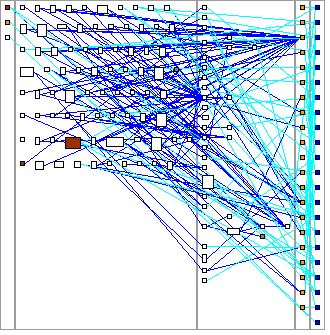
\includegraphics[width=\textwidth]{GLM_Presentation_blueprint}
\section{Correlation}
\newpage
\part{Conclusion}
\newpage
\part{Annexes}
\begin{figure}
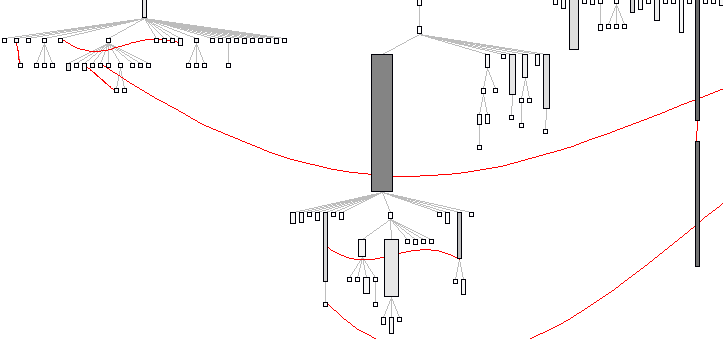
\includegraphics[width=\textwidth]{glamour_arch_dupli_1}
\label{arch_dupl_1}
\caption{Architecture with duplication links part 1}

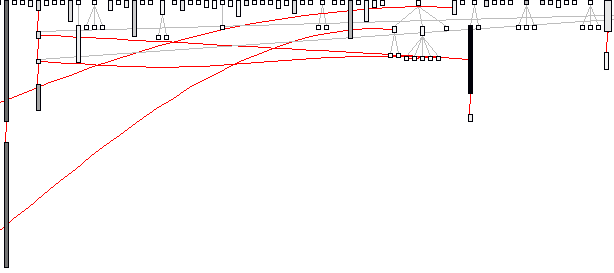
\includegraphics[width=\textwidth]{glamour_arch_dupli_3}
\label{arch_dupl_2}
\caption{Architecture with duplication links part 2}


\includegraphics[&]{glamour_arch_dupli_2}
\label{arch_dupl_3}
\caption{Architecture with duplication links part 3}

\end{figure}

\end{document}